%!TEX root = Report.tex

\section{Tracking}
This chapter is divided into three subparts. First we will introduce the reader to different image processesing techniques, and their uses. Following this we will introduce the reader to a framework that supports these techniques, and finish off by describing the implemened solution and the design choices.

% Gå ud fra at dette afsnit ikke har noget video input fra et kamera. Integration med kameraet kommer senere.
% 
% Teori først - hvilken slags image manipulation har vi brugt? hvad var alternativerne?
% Så framework - vi bruger OpenCV, why? hvad giver det os? hvad er drawbacks?
% så implementation - Hvad har vi implementeret? Hvordan var performance? hvad var vores alternativer? har vi eksperiementeret med nogen af de andre muligheder?
% 
% Image Segmentation - hvad giver det os/hvorfor er det smart?
% Thresholding
% Dilating
% Eroding
% Background detection and why we can't use it
% Alternatives and why we don't use them

\subsection{Theory}
This section will provide information about five common image processing techniques; thresholding, dilating and eroding, contrast, image segmentation and background filtering. The description of each technique will be backed up by examples. We will also use the \textit{ternary if} statement notation in this section which looks like the one shown in Equation \ref{eq:notation}.

\begin{equation}
value = {Boolean\mbox{-}Condition} ? {True\mbox{-}Evaluation}: {False\mbox{-}Evaluation}
\label{eq:notation}
\end{equation}

It works just like you would expect from many programming languages. It is also known as an inline \textit{if-statement}. \\

\noindent \textbf{Thresholding} \par
Thresholding is an image processing technique used to make a final decision about each pixel in an image. Either a pixel value is one that we are interested in or it is not. This is usually done by assigning a specific pixel value to the pixel we want, and another to those that we do not want. In general we compare the \textit{i}th pixel of the source image, \textit{src}, to the threshold value, \textit{T}, and saves the result in a destination image, \textit{dst}. For instance, to create a binary image where we are interested in all pixels above the threshold \textit{T}, the equation would look like the one shown in Equation \ref{eq:binarythresholding},

\begin{equation}
dst_i = src_i \geq T ? 255: 0
\label{eq:binarythresholding}
\end{equation}

Most threshold operations are applied on grayscale images, where all pixel values range between 0 (black) and 255 (white). Sometimes these values are normalized to range between 0 and 1 instead. However for the rest of this report we will assume that grayscale images use the former convention. Soon we will argue how thresholding can be expanded to also cover thresholding an RGB image. Figure \ref{fig:threshold_example} show an example of applying threshold to a grayscale image.

\begin{figure}
        \centering
        \begin{subfigure}[b]{0.3\textwidth}
                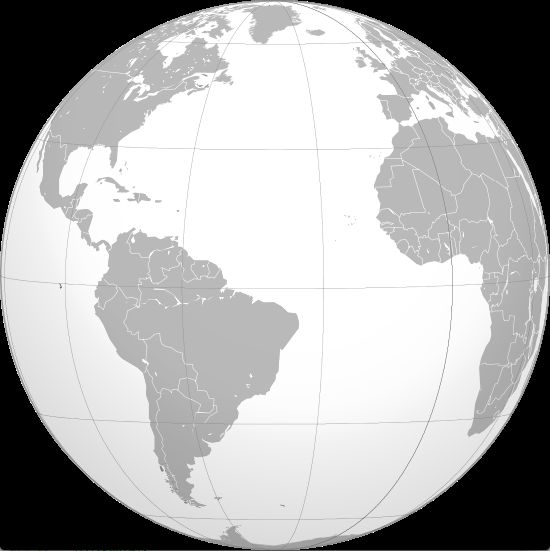
\includegraphics[scale = 0.2]{img/globe}
                \caption{Grayscale image}
        \end{subfigure}
		\quad
        \begin{subfigure}[b]{0.3\textwidth}
                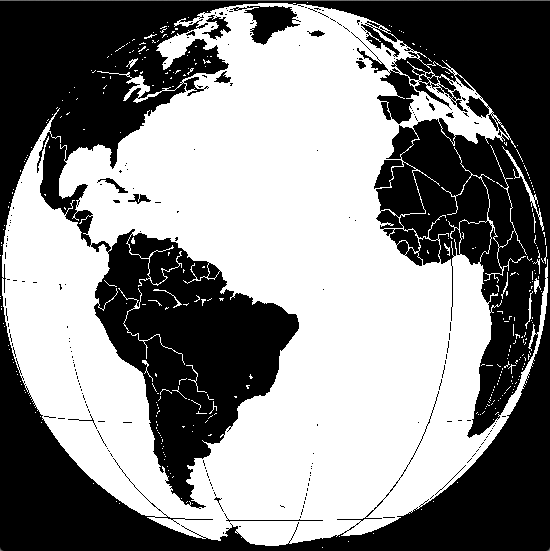
\includegraphics[scale = 0.2]{img/post_threshold}
                \caption{Thresholded image}
        \end{subfigure}
		\caption{An example of applying a threshold on a grayscale image. This example use the threshold value \textit{T} = 200}
		\label{fig:threshold_example}
\end{figure}

Now what happens if what you are interested in is a color? To use standard thresholding we first need to convert it to a grayscale image. However doing so might result in an image that have lost important information as can be seen in figure \ref{fig:RGB2GRAY}. Unless you want to find the red color, you have no way of differentiating the blue and green color.

\begin{figure}
        \centering
        \begin{subfigure}[b]{0.3\textwidth}
                
\includegraphics[scale=0.5]{img/RGB}
                \caption{RGB image}
        \end{subfigure}
		\quad
        \begin{subfigure}[b]{0.3\textwidth}
                
\includegraphics[scale=0.5]{img/GrayRGB}
                \caption{Grayscale image}
        \end{subfigure}
		\caption{Example of grayscaling a color image}
		\label{fig:RGB2GRAY}
\end{figure}

A step in the right direction would be to define the threshold value \textit{T} as a scalar consisting of three values - one for each color channel. We will denote this threshold scalar as \textit{S} and define it as shown in Equation \ref{eq:thresholdscalar}.

\begin{equation}
S =  
\begin{pmatrix}
  S_{R}\\
  S_{G}\\
  S_{B}\\
\end{pmatrix}
\label{eq:thresholdscalar}
\end{equation}

To apply it to an RGB image we need to change Equation \ref{eq:binarythresholding} to the one shown in Equation \ref{eq:threshold_RGB}.

\begin{equation}
{dst_i} = {src_i}_R \geq S_R \wedge {src_i}_G \geq S_G \wedge {src_i}_B \geq S_B? 255: 0
\label{eq:threshold_RGB}
\end{equation}

Trying it out makes it much easier to differentiate between colors. In Figure \ref{fig:RGB_Thresh} a threshold attemp using this method directly on the RGB image is shown.

\begin{figure}
        \centering
        \begin{subfigure}[b]{0.3\textwidth}
                
\includegraphics[scale=0.5]{img/RGB}
                \caption{RGB image}
        \end{subfigure}
		\quad
        \begin{subfigure}[b]{0.3\textwidth}
                
\includegraphics[scale=0.5]{img/RGBThresh}
                \caption{Thresholded image}
        \end{subfigure}
		\caption{Example of thresholding a color image with Equation \ref{eq:threshold_RGB} using the scalar \textit{S}=(0,100,0)}
		\label{fig:RGB_Thresh}
\end{figure}

However one issue remains - what if you want to find a color among similar colors? The problem is illustrated in Figure \ref{fig:green_fail} using the same scalar as in Figure \ref{fig:RGB_Thresh}

\begin{figure}
        \centering
        \begin{subfigure}[b]{0.3\textwidth}
                
\includegraphics[scale=0.5]{img/green}
                \caption{RGB image}
        \end{subfigure}
		\quad
        \begin{subfigure}[b]{0.3\textwidth}
                
\includegraphics[scale=0.5]{img/simpleRGBThresh}
                \caption{Thresholded image}
        \end{subfigure}
		\caption{Example of thresholding a color image with Equation \ref{eq:threshold_RGB} using the scalar \textit{S}=(0,100,0). Unlike before the result is unsatisfactory.}
		\label{fig:green_fail}
\end{figure}

The solution is to specify a \textit{range} of acceptable values instead of just a threshold. We will specify two scalars; S Upper, \textit{SU}, and S Lower, \textit{SL}.

\begin{equation}
SL =  
\begin{pmatrix}
  SL_{R}\\
  SL_{G}\\
  SL_{B}\\
\end{pmatrix}
\label{eq:thresholdlower}
\end{equation}

\begin{equation}
SU =  
\begin{pmatrix}
  SU_{R}\\
  SU_{G}\\
  SU_{B}\\
\end{pmatrix}
\label{eq:thresholdupper}
\end{equation}

We will use the definitions in Equations \ref{eq:thresholdlower} and \ref{eq:thresholdupper} to update Equation \ref{eq:threshold_RGB}. The changes can be seen in Equation \ref{eq:threshold_range}.

\begin{equation}
{dst_i} = SU_R \geq {src_i}_R \geq SL_R \wedge SU_G \geq {src_i}_G \geq SL_G \wedge SU_B \geq {src_i}_B \geq SL_B? 255: 0
\label{eq:threshold_range}
\end{equation}

Using a range to specify a color instead will yield a much more satisfactory result as shown in Figure \ref{fig:green_final}. \\

\begin{figure}
        \centering
        \begin{subfigure}[b]{0.3\textwidth}
                
\includegraphics[scale=0.5]{img/green}
                \caption{RGB image}
        \end{subfigure}
		\quad
        \begin{subfigure}[b]{0.3\textwidth}
                
\includegraphics[scale=0.5]{img/finalthresh}
                \caption{Thresholded image}
        \end{subfigure}
		\caption{Example of thresholding a color image with Equation \ref{eq:threshold_range} using the range \textit{SL}=(0,100,0) and \textit{SU}=(1,150,10). We have sucessfully located the dark green color area.}
		\label{fig:green_final}
\end{figure}

\noindent \textbf{Dilating and Eroding} \par
Forklar at vi har en kernel, B, med størrelsen s, der bliver anvendt på hver pixel, p, i et billede A.
Angiv at dilating finder local optima, og at eroding finder local minima.
Angiv at de her metoder bliver brugt EFTER thresholding for at "rense" billedet. \\

\begin{figure}[!ht]
        \centering
        \begin{subfigure}[b]{0.3\textwidth}
                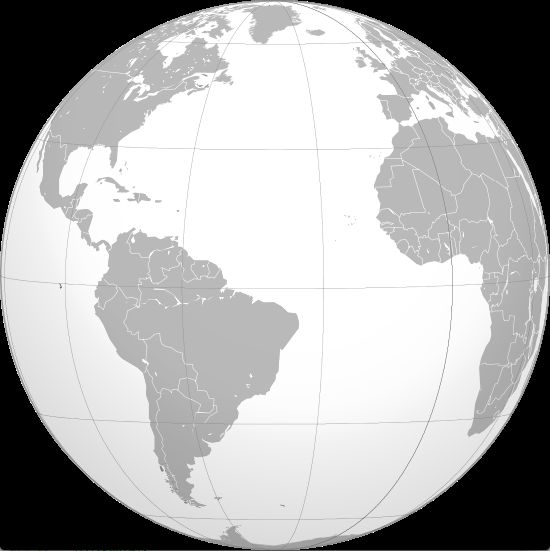
\includegraphics[scale = 0.2]{img/globe}
                \caption{Grayscale image}
        \end{subfigure}
		\quad
        \begin{subfigure}[b]{0.3\textwidth}
                
\includegraphics[scale = 0.2]{img/erode}
                \caption{Eroded image}
        \end{subfigure}
		\quad
        \begin{subfigure}[b]{0.3\textwidth}
                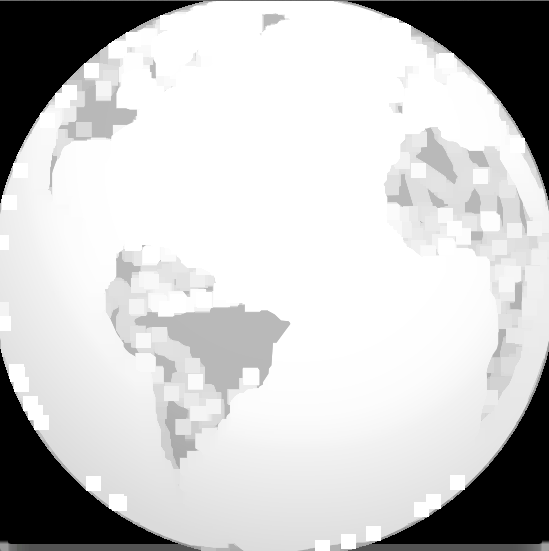
\includegraphics[scale = 0.2]{img/dilate}
                \caption{Dilated image}
        \end{subfigure}
		\caption{Eroding and dilating an image. It is clear that eroding expands dark areas and dilate expands bright areas. This example uses a 7x7 kernel.}
		\label{fig:erodedilate}
\end{figure}

\newpage

\noindent \textbf{Contrast} \par
Describe how $\alpha$ and $\beta$ is applied to each pixel in an image. \\

\noindent \textbf{Image Segmentation} \par
Describe how clustering algorithms is applied to create "pixel" blobs. \\

\noindent \textbf{Background Filtering} \par
Describe how computing the absolute difference in pixel values between two image filters out the background. \\

\subsection{Framework}
Describe OpenCV. Explain why it is preferable over other frameworks. \\

\subsection{Realization}
Describe the solution and design choices. E.g. why do we use thresholding but not Background Filtering. \\


